\documentclass[letterpaper, 11pt]{article}
%\usepackage[round]{natbib}


\usepackage{pdfpages}
\usepackage{mathtools}
\usepackage{setspace} 
\usepackage{dsfont}
\usepackage{amsfonts}
\usepackage{amsmath}
\usepackage{subcaption}
\usepackage{paralist}
%\usepackage{subfig}
\usepackage{times}
\usepackage{latexsym}
\usepackage{graphicx}
\usepackage[T1]{fontenc}
\usepackage{tikz}
\usepackage{url}
\usepackage{pgfplotstable}
\usepackage{titlesec}
\usepackage{color}
\usepackage{lipsum,adjustbox}
\usepackage[font={small}]{caption}
\usetikzlibrary{positioning}
\usepackage{bbm}

\makeatletter
\newcommand{\@BIBLABEL}{\@emptybiblabel}
\newcommand{\@emptybiblabel}[1]{}
%\makeatother
\usepackage[hidelinks]{hyperref}


\usepackage{acl2012}
\graphicspath{{../plots/}}
\newcommand{\com}[1]{}
%\newcommand{\oa\part{title}}[1]{}
%\newcommand{\lc}[1]{}
\newcommand{\oa}[1]{\footnote{\color{red}OA: #1}}
\newcommand{\oamod}[1]{{\color{red}#1}}
\newcommand{\lc}[1]{\footnote{\color{blue}LC: #1}}
\newcommand{\lcmod}[1]{{\color{blue}#1}}

\newenvironment{myequation}{
  \vspace{-1em}
 \begin{equation}
}{
 \end{equation}
 \vspace{-1.2em}
}
\newenvironment{myequation*}{
	\vspace{-1em}
	\begin{equation*}
}{
\end{equation*}
\vspace{-1.2em}
}


\begin{document}

\title{41808: Issues in typology:\\Defining language families by phonemes}
\author{
  Leshem Choshen \\
  \textsuperscript{1}School of Computer Science and Engineering,
  \textsuperscript{2} Department of Cognitive Sciences \\
  The Hebrew University of Jerusalem \\
  \texttt{leshem.choshen@mail.huji.ac.il}\\
}
\maketitle
\section{Introduction}
Language families are used through all fields of linguistics, questions are being asked about the differences between specific families and the differences between specific languages in them. We wish to raise the question of how are language families actually defined, and in the same breath admit that they are not. Knowing the definition of families is based on intuition that relies on countless factors such as history, lexicons, cognition and phonetics, we wish to compare various phonemic based automatic methods to help us better understand at least the phonetic aspects we rely upon or should rely upon when we make the decisions about language families. This paper conducts two main experiments evaluating automatic measures for language clusterings, finding phonemes to be more reliable than phonemic features as a space in which languages should be compared, and suggesting metric learning as a better way than any of the rule-based distance metrics. The second experiment included ordering different sets of features showing which features tend to signify two languages come from different families and which features tend to diverge more, without being of different origins.
\section{Relevant background}
As we use different computational tools and terms that some readers might not be familiar with, we wish to explain and define a few.
\paragraph{Edit distance} between two phonemes is the minimal amount of actions in the form of adding or deleting a feature of a phoneme to get one phoneme to be identical to the other. In terms of computation, edit distance is calculated by the count of features that are found exactly in one of the two phonemes.
\paragraph{Bipartite graph} is a graph in which two sets of nodes exist which have edges only between the sets and not between edges in the same set.
\begin{figure*}
	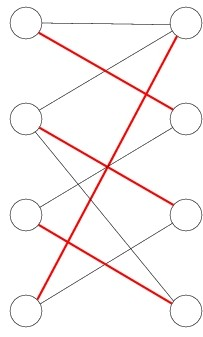
\includegraphics[width=0.8\columnwidth]{Matching_pic_3_1_and_3_2}
	\caption{Bipartite graph match
		\label{fig:bipartite}
	}
\end{figure*}
\paragraph{Bipartite graph matching}  - given a bipartite graph the goal is to look for the maximum matching. I.e. finding a set with the maximum number of edges such that each node is connected at most once. If there are weights on the edges, a specific such set might be sought after, usually one with the maximum or minimum sum of weights.
Metric learning is an area of supervised machine learning where the goal is to learn from examples a distance function that measures how similar or related two objects are. 

As far as linguistics background is concerned, we might note that language families are found in many linguistic studies \cite{aikhenvald1999arawak} and sophisticated automatic tools were already used for various related tasks \cite{bouckaert2012mapping}. We do not know of other attempts to confront language proximity in terms of phonemic inventory and a comparison of automatic ways to do so. 
Phonemic inventories have the advantage of being available in many languages and dialects and are also structured, allowing for meaningful comparison. This drives us to look for a better use of phoneme inventories in language comparison and in creating measures to assess language families using phonemic inventories. Despite those advantages, as an exact definition of language family is hard to get by, as phonemic inventories tend to change more than phonetic rules and syntax \cite{mohammadi2comparative} and as there are many parameters with which to compare and data is relatively scarce, this is a challenging task.
\section{Methods}
\paragraph{Data} Throughout this paper we use two datasets, the Kurdistan dataset created in class and the Eurasia database \cite{Nikolaev2015database}. We combine the two datasets using the fields Group and the broader gen subfield respectively to represent language families. Language families containing 4 or less languages were dropped from our experiments.
\footnote{All code is freely available and can be found in https://github.com/borgr/languageClustering}

The first part of the project was to try and automatically divide languages to families based on their phonological inventories. More specifically, diana divisive hierarchical clustering algorithm was used and the research question was which distance measure could be used to compare language inventories well, assuming that, generally, the phoneme inventory is sufficient to classify a language to its family. The proposed metrics that were created were based on three representation types, or three projections to n-dimensional spaces; Binary - a representation of the phonemes that existed in the language, bag of features - a positive integer representation counting the number of times each feature (e.g. “tap”) was found in the phonemes of the inventory and bag of n-grams - (n=2 was used to avoid too many features) containing the counts of phonemes that have the specific n-tuple features (e.g. having the phoneme d would add 1, among others, to the count of “alveolar + plosive”). After projecting to these spaces, conventional metrics may be used (euclidean, cosine similarity etc.), choosing the right metric, even given a representation, is not an easy task by itself and many options exist. Thus, distances were chosen to cover different types of distance metrics\cite{cha2007comprehensive,choi2010survey}, specifically for binary representations Hamming, Jaccard and Yole distances were used and for non binary cosine and euclidean.
Another approach in the direction of choice over distances was metric learning. With manual choice of a metric we may always be in doubt that perhaps the interesting information is well represented in our current features, but we chose an inappropriate metric. For that reason half of the languages were randomly assigned for evaluation to ITML \cite{davis2007information}, a metric learning algorithm. Many other metric learning methods \cite{shental2002adjustment} were tested and dropped due to technicalities, mainly ones concerning the small number of instances of certain classes (language families) in the database.
Lastly, a distance of a different flavor was used, inspired by the work of \newcite{macklin2015high}. It was not based on any vector space. Instead, to compute the distance between two phoneme inventories, an alignment of the most similar phonemes was done and the total edit distance of features was used. Alignment is done by reformulating the problem as finding a bipartite graph match with minimal weights, the edit distance is considered to be the weights between phonemes of the two compared languages. Using Kuhn Munkres algorithm we can efficiently find the best solution.

A second part of the project was to assess which features are especially good for differentiating families of languages. For that I have used feature elimination tests using the 3 different sets of features spanning our spaces; letters, feature unigrams, feature bigrams. These tests give us a rank over the features telling us which feature is the most useful for  classification. 
Technically, it is a repetitive fitting of a machine learning classifier, in our case logistic regression, again and again, each time removing the least important feature from the list of available features for classification. 
Linguistically, if a feature is ranked higher it means it is a better measure to determine languages are of different family, and if it is low, it is either rare or as frequent in one family as in another, suggesting it might be a common thing that is added\textbackslash\{\}removed from the language by phonemic change or contact and not something that if added is stable across the generations and stays in many of the family’s languages. 
\section{Disadvantages of the suggested methods and further work}
\begin{itemize}
	\item We obviously do not have a good representation of most of the language families, but we have enough for general conclusions.
	\item It is not unlikely that an ingenious distance metric exists that will be much better than any of the ones introduced here, that might be considered further work.
	\item Hierarchical clustering comparison was done mainly by visualization. Quantitative measures, such as validating indexes are a possible tool even though they add another significant time consuming part to the project and fit non-hierarchical clustering better.
	\item Our held-out data is per language, so perhaps a better approach for a train test method was to hold full language families out and to see what happens then, can metric learning methods generalize differences in language families they did not train with.
	\item Are the same features and distances the best when separating eurasia languages from kurdish languages?
	\item As this was only an initial step subcategories that existed (for eurasia languages only) were not used to specify that languages inside a family are closer in terms of distance, but that will produce more data and  surely make the metrics much more robust. Some metric learning algorithms get as input tuples of dist(X[a],X[b]) < dist(X[c],X[d]) where X data and a,b,c,d indices, for those we can use both groups and subgroups of languages as we know the relations. Other metrics only deal with equivalence classes as input and thus can not benefit from this information.
	\item In the scenario of metric learning we have a problematic split between validation and test, 50\% of the languages in the test were the training data. Other distances do not train and thus have no such problems.
\end{itemize}
\section{Analysis and findings}
Clustering results show that alignment, bag of features and n-gram representations all fail to create reasonable metrics, with many of the phoneme inventories not necessarily from the same family having the exact same distances from each other and so being clustered together in large groups. Using binary representation and comparing with Hamming distance or Jaccard (not Yole), we see results which are quite promising. The plots in Appendix B show that the phonemes themselves have more information than the relaxations created for this experiment and that the information can be used as is.
We may carefully deduce from the failure of the alignment distance that although phonemes may change gradually, some small features are not as easily changed, and to make a good comparison aspects of the way each feature change must be carefully studied and weighted.
Results from learning to rank are not only a possible direction to look for metrics, they can also tell us how good are our extracted features, we base our features on the thought that the phonetic features are a fact and the only way to classify phonemes (and perhaps they are), but are they the right features to look at on this problem? The results we get suggested they might not be. With half the data to train on, ITML is doing quite well, many of the families indeed get their own clusters. It seems it is doing even better than the binary phonemic inventory representation, as can be seen for example in the nice clustering it gives to Tai-kadai. 
This might be the place to address the fact that we still see the difficulty of the problem and witness the groups that are separated to smaller clusters and the languages that are attached to the wrong cluster of languages.

See Appendix C for the full rankings of the features. From the results over feature selection we can see that the glottal and pharyngeal as well as the phonemes 'ʔ', 'ʕ' are high in the list of features, it is a sign that at least something expected is happening in the feature selection. Originally we were looking at the languages of Kurdistan, among those it is a significant sign of Arabic, which, to my knowledge is rare in other language families such as the Indo-Iranian. We also see various phonemes similar to ‘ts’ being very distinctive, perhaps suggesting they don’t tend to be adopted, while common and hardly changing ‘b’ is relatively low in the list.
Most humbly I do not pretend to know enough to be able to analyze the results in this part well by myself, and they call for a linguist with more phonetic background to have a more insightful say about them.
\appendix
\section{Executing}
If the results are not found and you wish to calculate them by yourself note the following things:
\begin{itemize}
	\item It might be faster to ask leshem.choshen@mail.huji.ac.il for the caches as the two levels of cache (db and distance matrix) make things much faster.
	\item  The main python file “binarize\_representations.py contains mains of the two parts
	\item calculate\_distances\_main(inv\_db, feature\_db, base\_db)
	\item choose\_features\_main(inv\_db, feature\_db, base\_db)
	\item  It may be the case you only wish to run one of those.
	\item Running of the distance main may require a lot of processing time, and for distance learning multithreading is done. Running everything from scratch may take a day of computing.
	\item Given that you have computed the distance matrices you want to plot (copied or ran the main), run the R file hierarchy\_option2.R to create the plots
\end{itemize}

\section{Dendrograms}
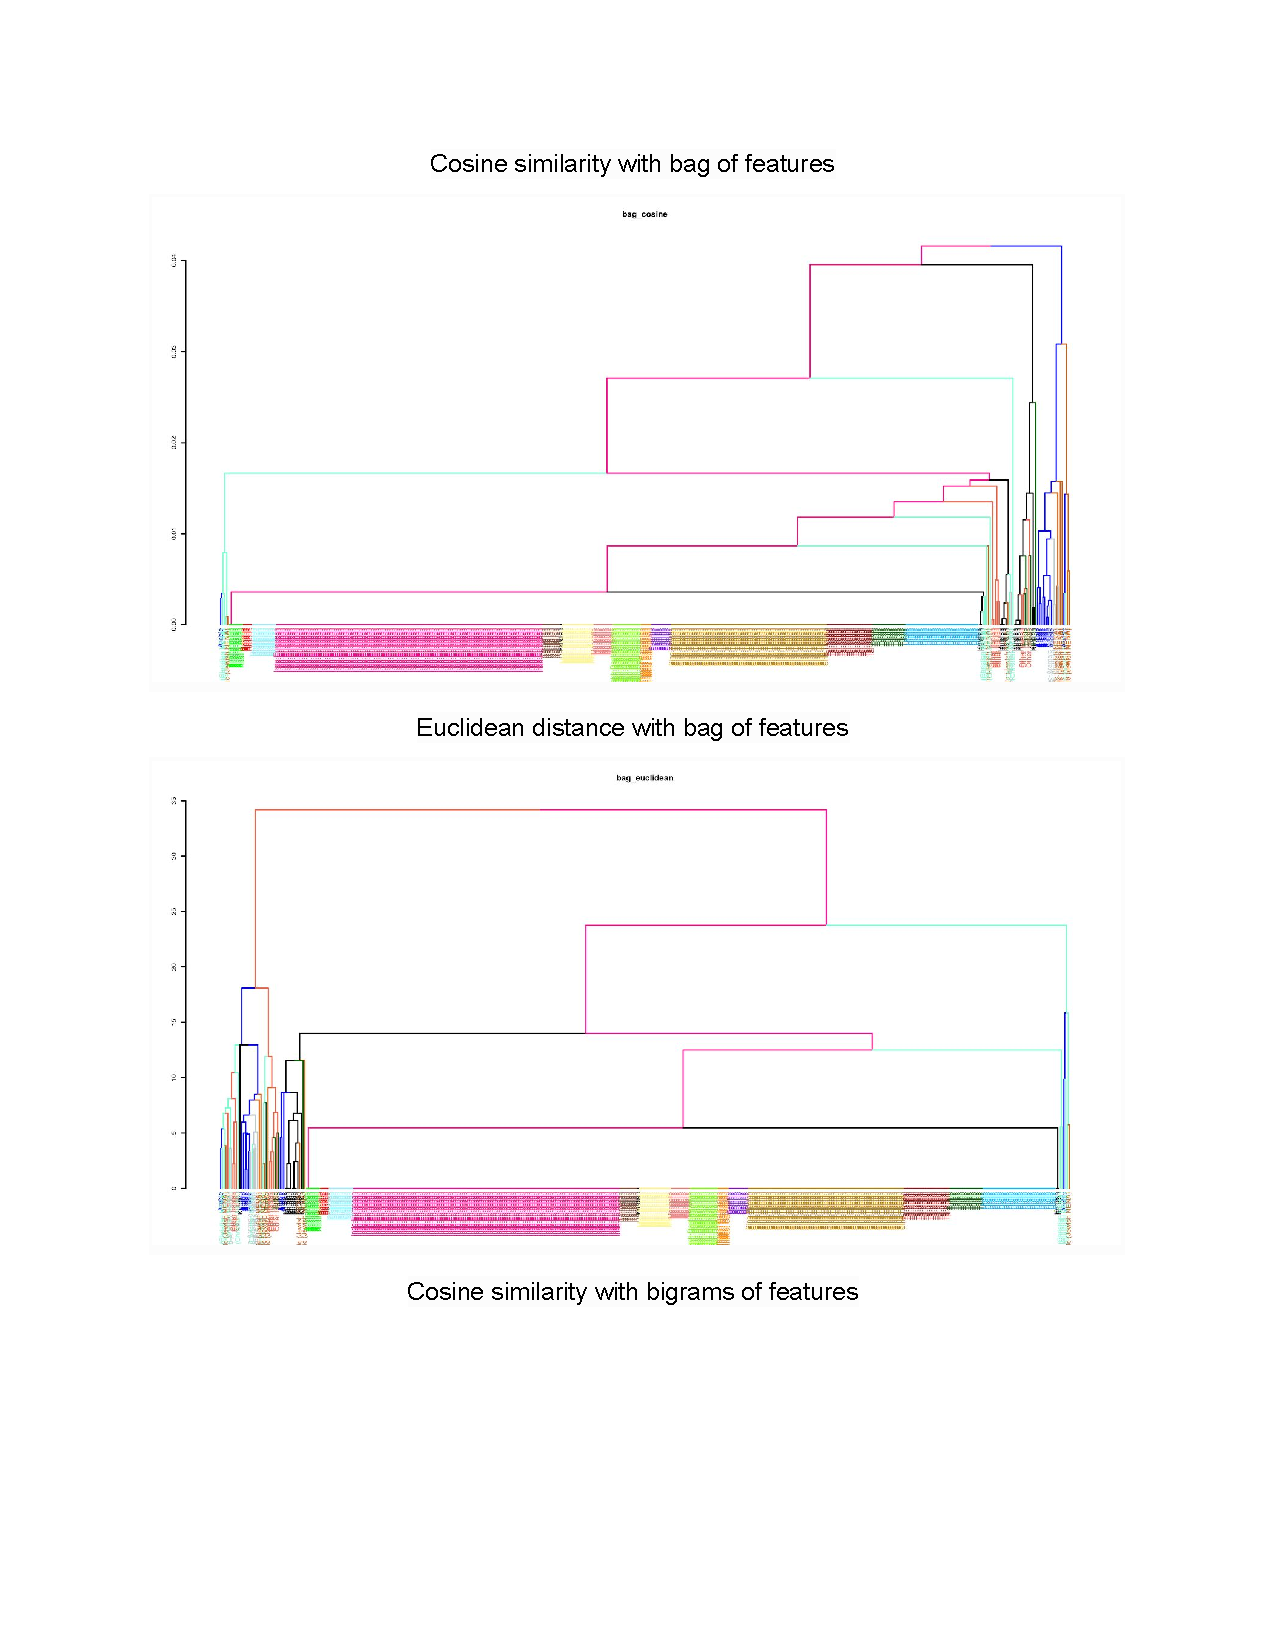
\includepdf[pages=-,offset=0mm 6mm]{dends.pdf}
\section{Feature ranking}
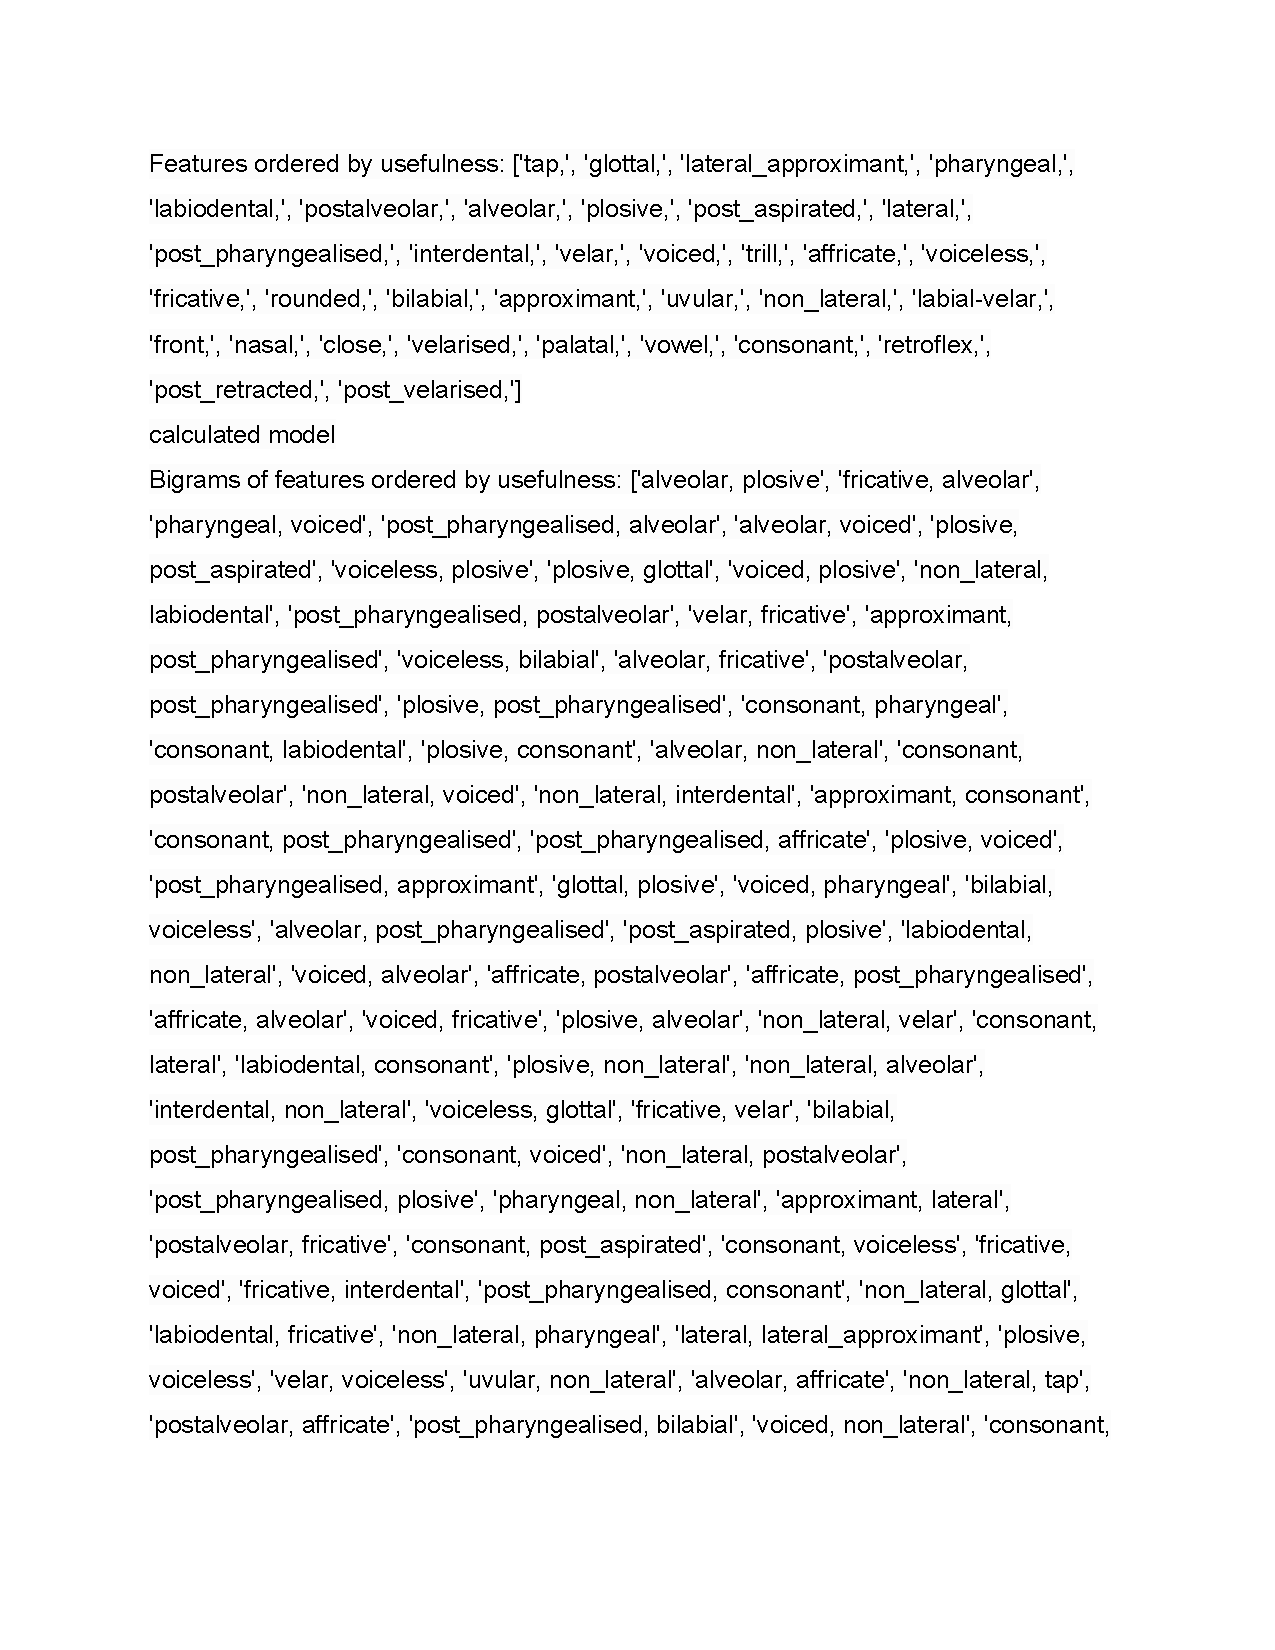
\includepdf[pages=-,offset=0mm 6mm]{rank.pdf}

\bibliographystyle{acl2012}
\bibliography{cites}

\end{document}
